\documentclass[journal,12pt,twocolumn]{IEEEtran}
%
\makeatletter
\makeatother
\usepackage{setspace}
\usepackage{gensymb}
\usepackage{xcolor}
\usepackage{caption}
%\usepackage{stackengine}
%\usepackage{subcaption}
%\doublespacing
\singlespacing



\usepackage{graphicx}
\graphicspath{ {./images}  }
%\usepackage{amssymb}
%\usepackage{relsize}
\usepackage[cmex10]{amsmath}
\usepackage{mathtools}
%\usepackage{amsthm}
\interdisplaylinepenalty=2500
%\savesymbol{iint}
%\usepackage{tikz}
%\usepackage{txfonts}
%\restoresymbol{TXF}{iint}
\usepackage{wasysym}
\usepackage{amsthm}
\usepackage{mathrsfs}
\usepackage{txfonts}
\usepackage{stfloats}
\usepackage{cite}
\usepackage{cases}
\usepackage{mathtools}
\usepackage{subfig}
\usepackage{enumerate}	
\usepackage{enumitem}
\usepackage{amsmath}
%\usepackage{xtab}
\usepackage{longtable}
\usepackage{multirow}
%\usepackage{algorithm}
%\usepackage{algpseudocode}
\usepackage{enumitem}
\usepackage{mathtools}
%\usepackage{iithtlc}
%\usepackage[framemethod=tikz]{mdframed}
\usepackage{tikz}
\usetikzlibrary{positioning}
\usepackage{listings}
\usepackage{listings}
    \usepackage[latin1]{inputenc}                                 %%
    \usepackage{color}                                            %%
    \usepackage{array}                                            %%
    \usepackage{longtable}                                        %%
    \usepackage{calc}                                             %%
    \usepackage{multirow}                                         %%
    \usepackage{hhline}                                           %%
    \usepackage{ifthen}                                           %%
  %optionally (for landscape tables embedded in another document): %%
    \usepackage{lscape}     



%\usepackage{stmaryrd}


%\usepackage{wasysym}
%\newcounter{MYtempeqncnt}
\DeclareMathOperator*{\Res}{Res}
%\renewcommand{\baselinestretch}{4}
%\setcounter{secnumdepth}{4}
\renewcommand\thesection{\arabic{section}}
\renewcommand\thesubsection{\thesection.\arabic{subsection}}
\renewcommand\thesubsubsection{\thesubsection.\arabic{subsubsection}}
%\renewcommand\thesubsubsubsection{\thesubsubsection.\arabic{subsubsubsection}}

%\renewcommand\thesectiondis{\arabic{section}}
%\renewcommand\thesubsectiondis{\thesectiondis.\arabic{subsection}}
%\renewcommand\thesubsubsectiondis{\thesubsectiondis.\arabic{subsubsection}}
%\renewcommand\thesubsubsubsectiondis{\thesubsubsectiondis.\arabic{subsubsubsection}}
% correct bad hyphenation here
\hyphenation{op-tical net-works semi-conduc-tor}

%\lstset{
%language=C,
%frame=single, 
%breaklines=true
%}

%\lstset{
	%%basicstyle=\small\ttfamily\bfseries,
	%%numberstyle=\small\ttfamily,
	%language=Octave,
	%backgroundcolor=\color{white},
	%%frame=single,
	%%keywordstyle=\bfseries,
	%%breaklines=true,
	%%showstringspaces=false,
	%%xleftmargin=-10mm,
	%%aboveskip=-1mm,
	%%belowskip=0mm
%}

%\surroundwithmdframed[width=\columnwidth]{lstlisting}
\def\inputGnumericTable{}                                 %%

\lstset{
%language=python,
frame=single, 
breaklines=true,
columns=fullflexible
}

 

\begin{document}
%

\theoremstyle{definition}
\newtheorem{theorem}{Theorem}[section]
\newtheorem{problem}{Problem}
\newtheorem{proposition}{Proposition}[section]
\newtheorem{lemma}{Lemma}[section]
\newtheorem{corollary}[theorem]{Corollary}
\newtheorem{example}{Example}[section]
\newtheorem{definition}{Definition}[section]
%\newtheorem{algorithm}{Algorithm}[section]
%\newtheorem{cor}{Corollary}
\newcommand{\BEQA}{\begin{eqnarray}}
\newcommand{\EEQA}{\end{eqnarray}}
\newcommand{\define}{\stackrel{\triangle}{=}}

\bibliographystyle{IEEEtran}
%\bibliographystyle{ieeetr}

\providecommand{\nCr}[2]{\,^{#1}C_{#2}} % nCr
\providecommand{\nPr}[2]{\,^{#1}P_{#2}} % nPr
\providecommand{\mbf}{\mathbf}
\providecommand{\pr}[1]{\ensuremath{\Pr\left(#1\right)}}
\providecommand{\qfunc}[1]{\ensuremath{Q\left(#1\right)}}
\providecommand{\sbrak}[1]{\ensuremath{{}\left[#1\right]}}
\providecommand{\lsbrak}[1]{\ensuremath{{}\left[#1\right.}}
\providecommand{\rsbrak}[1]{\ensuremath{{}\left.#1\right]}}
\providecommand{\brak}[1]{\ensuremath{\left(#1\right)}}
\providecommand{\lbrak}[1]{\ensuremath{\left(#1\right.}}
\providecommand{\rbrak}[1]{\ensuremath{\left.#1\right)}}
\providecommand{\cbrak}[1]{\ensuremath{\left\{#1\right\}}}
\providecommand{\lcbrak}[1]{\ensuremath{\left\{#1\right.}}
\providecommand{\rcbrak}[1]{\ensuremath{\left.#1\right\}}}
\theoremstyle{remark}
\newtheorem{rem}{Remark}
\newcommand{\sgn}{\mathop{\mathrm{sgn}}}
\providecommand{\abs}[1]{\left\vert#1\right\vert}
\providecommand{\res}[1]{\Res\displaylimits_{#1}} 
\providecommand{\norm}[1]{\lVert#1\rVert}
\providecommand{\mtx}[1]{\mathbf{#1}}
\providecommand{\mean}[1]{E\left[ #1 \right]}
\providecommand{\fourier}{\overset{\mathcal{F}}{ \rightleftharpoons}}
%\providecommand{\hilbert}{\overset{\mathcal{H}}{ \rightleftharpoons}}
\providecommand{\system}{\overset{\mathcal{H}}{ \longleftrightarrow}}
	%\newcommand{\solution}[2]{\textbf{Solution:}{#1}}
\newcommand{\solution}{\noindent \textbf{Solution: }}
\providecommand{\dec}[2]{\ensuremath{\overset{#1}{\underset{#2}{\gtrless}}}}
\DeclarePairedDelimiter{\ceil}{\lceil}{\rceil}
%\numberwithin{equation}{subsection}
\numberwithin{equation}{section}
%\numberwithin{problem}{subsection}
%\numberwithin{definition}{subsection}
%\makeatletter
%\@addtoreset{figure}{section}
%\makeatother

\let\StandardTheFigure\thefigure
%\renewcommand{\thefigure}{\theproblem.\arabic{figure}}
%\renewcommand{\thefigure}{\thesection}


%\numberwithin{figure}{subsection}

%\numberwithin{equation}{subsection}
%\numberwithin{equation}{section}
%\numberwithin{equation}{problem}
%\numberwithin{problem}{subsection}
%\numberwithin{problem}{section}
%%\numberwithin{definition}{subsection}
%\makeatletter
%\@addtoreset{figure}{problem}
%\makeatother
%\makeatletter
%\@addtoreset{table}{problem}
%\makeatother

\let\StandardTheFigure\thefigure
\let\StandardTheTable\thetable
%%\renewcommand{\thefigure}{\theproblem.\arabic{figure}}
%\renewcommand{\thefigure}{\theproblem}

%%\numberwithin{figure}{section}

%%\numberwithin{figure}{subsection}



\def\putbox#1#2#3{\makebox[0in][l]{\makebox[#1][l]{}\raisebox{\baselineskip}[0in][0in]{\raisebox{#2}[0in][0in]{#3}}}}
     \def\rightbox#1{\makebox[0in][r]{#1}}
     \def\centbox#1{\makebox[0in]{#1}}
     \def\topbox#1{\raisebox{-\baselineskip}[0in][0in]{#1}}
     \def\midbox#1{\raisebox{-0.5\baselineskip}[0in][0in]{#1}}




\title{ 
%	\logo{
Implementation of Low Density Parity Check (LDPC) codes
%	}
}



\author{Theresh Babu Benguluri, Sandeep Kumar Khyalia and G V V Sharma$^{*}$% <-this % stops a space
\thanks{*The author is with the Department
of Electrical Engineering, Indian Institute of Technology, Hyderabad
502285 India e-mail:  gadepall@iith.ac.in.}
}


% make the title area
\maketitle

\tableofcontents

%\bigskip
%
\begin{abstract}
\boldmath
A brief description about the design and implementataion of LDPC codes using (7,4) Hamming parity check matrix.
\end{abstract}


%\IEEEpeerreviewmaketitle

\section{Introduction}
Let the Channel model be,
\begin{equation}
Y_k= X_k + V_k, \quad k = 0,\dots,6
\end{equation} 
where $X_k$ is the  transmitted symbol in the $k$th time slot using the BPSK modulation and $V_k(m) \sim \mathcal{N}\brak{0,\sigma^2} $. 

\section{Encoding}
 LDPC codes are popular linear block codes with closest shannon limt channel capacity \cite{ldpc}. As an example Lets take (7,4) Hamming parity check matrix.
 \begin{equation} \label{eq:H}
 H =  \begin{bmatrix} 
1 & 1 & 1 & 0 & 1 & 0 & 0 \\
1 & 0 & 1 & 1 & 0 & 1 & 0 \\
1 & 1 & 0 & 1 & 0 & 0 & 1 
\end{bmatrix}
 \end{equation}

Above $H$ matrix having the parameters, information bits $k=4$ i.e $m=m_0,\dots,m_3$ , parity bits are $m=n-k=3$ i.e $p=[p_0,p_1,p_2]$ and  code word length $n=7$ i.e $c=[m\hspace{1mm}p]$.
\begin{figure}[!ht]
\begin{center}
%\begin{tikzpicture}
%
%    \node[shape=circle,draw=black] (v6) at (0,0) {v6};
%    \node[shape=circle,draw=black] (v5) at (0,1) {v5};
%    \node[shape=circle,draw=black] (v4) at (0,2) {v4};
%    \node[shape=circle,draw=black] (v3) at (0,3) {v3};
%    \node[shape=circle,draw=black] (v2) at (0,4) {v2};
%    \node[shape=circle,draw=black] (v1) at (0,5) {v1};
%    \node[shape=circle,draw=black] (v0) at (0,6) {v0};
%
%    
%
%
%    \node[shape=rectangle,draw=black] (p0) at (4,5) {p0};
%    \node[shape=rectangle,draw=black] (p1) at (4,3) {p1};
%    \node[shape=rectangle,draw=black] (p2) at (4,1) {p2};
%
%\path [-] (v0) edge node[left] {} (p0);
%\path [-] (v0) edge node[left] {} (p1);
%\path [-] (v0) edge node[left] {} (p2);
%\path [-] (v1) edge node[left] {} (p0);
%\path [-] (v1) edge node[left] {} (p2);
%\path [-] (v2) edge node[left] {} (p0);
%\path [-] (v2) edge node[left] {} (p1);
%\path [-] (v3) edge node[left] {} (p1);
%\path [-] (v3) edge node[left] {} (p2);
%\path [-] (v4) edge node[left] {} (p0);
%\path [-] (v5) edge node[left] {} (p1);
%\path [-] (v6) edge node[left] {} (p2);
%
%\path [->] (-1,0) edge node[left] {} (v6);
%\path [->] (-1,1) edge node[left] {} (v5);
%\path [->] (-1,2) edge node[left] {} (v4);
%\path [->] (-1,3) edge node[left] {} (v3);
%\path [->] (-1,4) edge node[left] {} (v2);
%\path [->] (-1,5) edge node[left] {} (v1);
%\path [->] (-1,6) edge node[left] {} (v0);
%
%\node[] at (-1.7,0) {$L(6)$};
%\node[] at (-1.7,1) {$L(5)$};
%\node[] at (-1.7,2) {$L(4)$};
%\node[] at (-1.7,3) {$L(3)$};
%\node[] at (-1.7,4) {$L(2)$};
%\node[] at (-1.7,5) {$L(1)$};
%\node[] at (-1.7,6) {$L(0)$};
%
%\node[] at (0,7) {variable nodes};\\
%\node[] at (4,7) {check nodes};\\
%\end{tikzpicture}
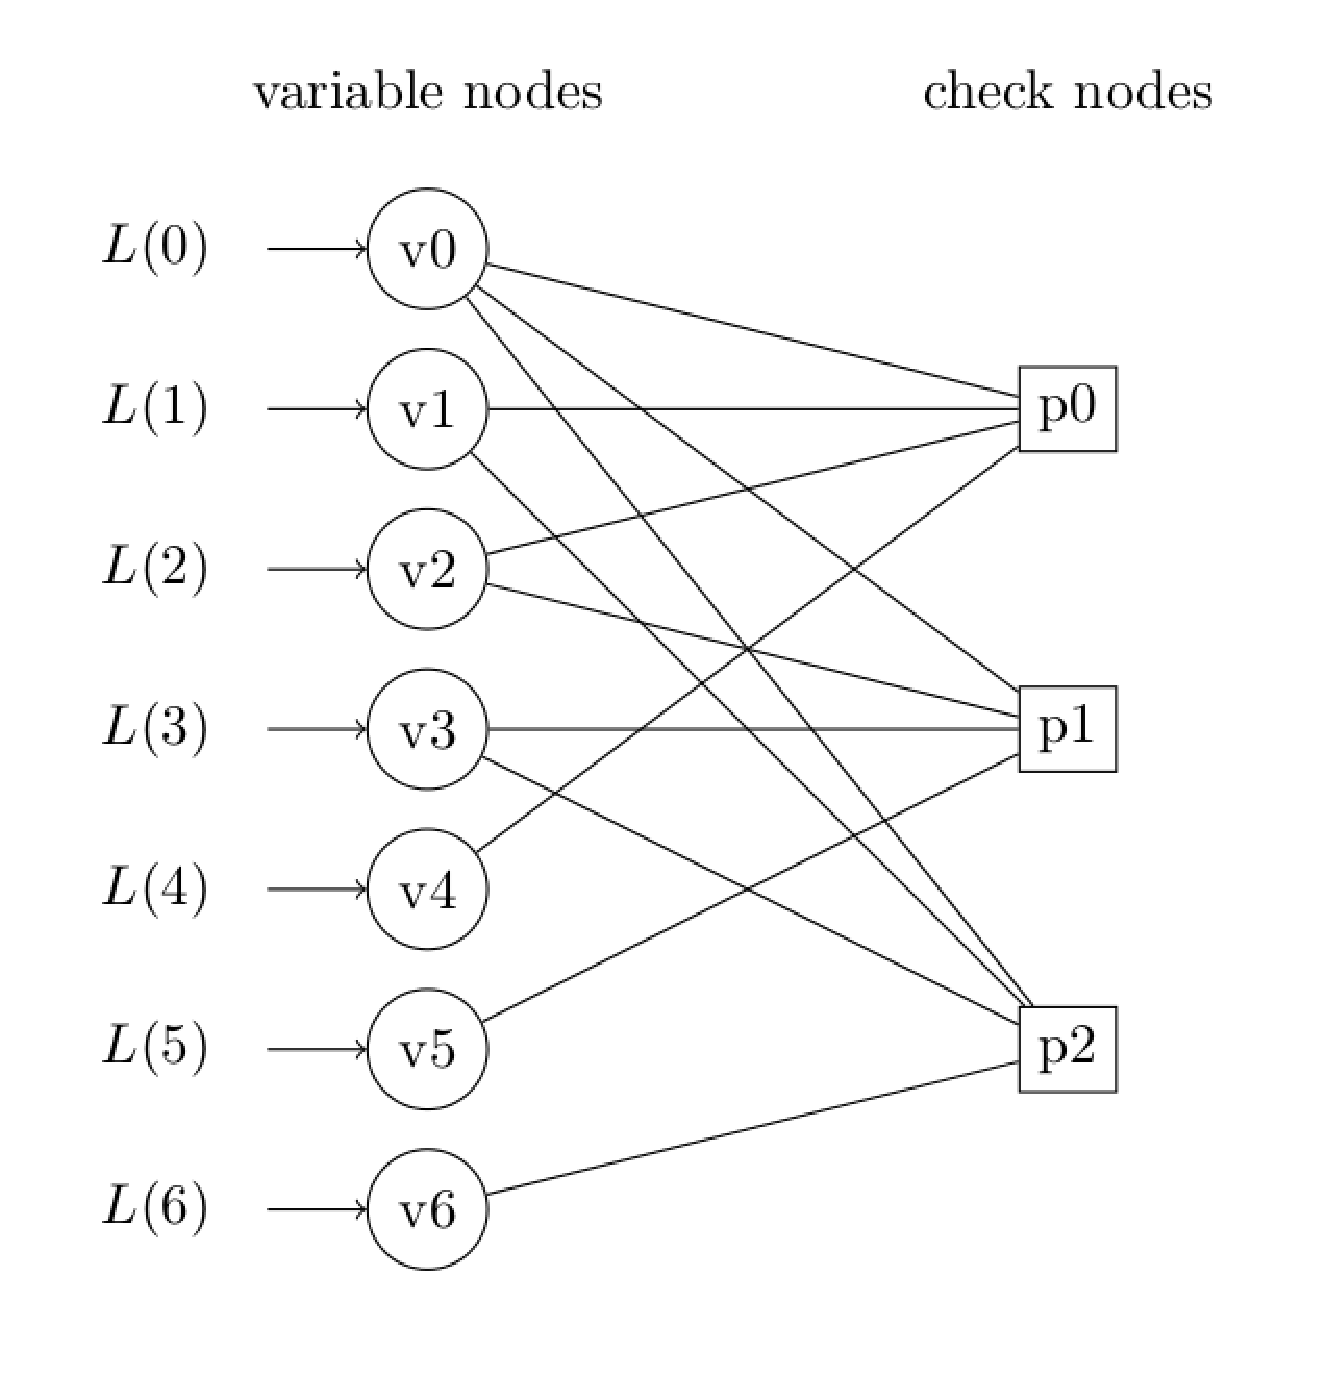
\includegraphics[width=\columnwidth]{./figs/tanner}
\caption{Tanner Graph Representation for (7,4) Hamming parity check matrix}
\label{fig:tanner}
\end{center}
\end{figure}
Encoding can be carried out by using 
\begin{align}
H &\times c^T =0 \\
 \begin{bmatrix} 
1 & 1 & 1 & 0 & 1 & 0 & 0 \\
1 & 0 & 1 & 1 & 0 & 1 & 0 \\
1 & 1 & 0 & 1 & 0 & 0 & 1 
\end{bmatrix} &  \begin{bmatrix} 
m_0\\
m_1\\
m_2\\
m_3 \\
p_0 \\
p_1\\
p_2
\end{bmatrix} = 0
\end{align}
solving we get
\begin{align}
p_0 &= m_0 \oplus m_1 \oplus m_2 \\
p_1 &= m_0 \oplus m_2 \oplus m_3 \\
p_2 &= m_0 \oplus m_1 \oplus m_3 
\end{align}
This is called Systematic Encoding.i.e Encoder will ensures information bits followed by parity bits.
\section{Decoding}
\subsection{Useful Calculations for proceeding LDPC Decoding }
\begin{enumerate}
\item Calculation of Input Channel Log Likelihood Ratio LLR 
\begin{align}
L(x_j)&=\log \brak{\frac{Pr(x_j=1|y)}{Pr(x_j=-1|y)}} \quad X=1-2c\\
&= \log \brak{\frac{f(y|x_j=1)Pr(x_j=1)}{f(y|x_j=-1)Pr(x_j=-1)}} \\
&= \log \brak{\frac{\frac{1}{\sqrt{2\pi\sigma^2}}e^{\frac{-(y_j-1)^2}{2\sigma^2}}}{\frac{1}{\sqrt{2\pi\sigma^2}}e ^{\frac{-(y_j+1)^2}{2\sigma^2}}} } \\
&=\log \brak{e^{\frac{2y_j}{\sigma^2}}} \\
L(x_j)&= \frac{2y_j}{\sigma^2} \label{eq :li}
\end{align}
\item Check Node Operation : \\
Lets assume that we have initilized all LLR values to variable nodes and we sent to check nodes. ${V_j}$ represents all the variable nodes which are connected to $j^{th}$ check node. Using the min-sum approximation\cite{minsum}, the message from  $j^{th}$ check node to  $i^{th}$ variable node given by,
\begin{figure}[!ht]
\begin{center}
%\begin{tikzpicture}
%    \node[shape=circle,draw=black] (v4) at (0,3) {v4};
%
%    \node[shape=circle,draw=black] (v2) at (0,4) {v2};
%    \node[shape=circle,draw=black] (v1) at (0,5) {v1};
%    \node[shape=circle,draw=black] (v0) at (0,6) {v0};
%
%    \node[shape=rectangle,draw=black] (p0) at (3,5) {p0};
%
%\path [<-] (v0) edge node[left] {} (p0);
%
%\path [->] (v1) edge node[left] {} (p0);
%
%\path [->] (v2) edge node[left] {} (p0);
%
%\path [->] (v4) edge node[left] {} (p0);
%
%
%
%\path [->] (-1,3) edge node[left] {} (v4);
%\path [->] (-1,4) edge node[left] {} (v2);
%\path [->] (-1,5) edge node[left] {} (v1);
%\path [->] (-1,6) edge node[left] {} (v0);
%
%
%\node[] at (-1.7,3) {$L(4)$};
%\node[] at (-1.7,4) {$L(2)$};
%\node[] at (-1.7,5) {$L(1)$};
%\node[] at (-1.7,6) {$L(0)$};
%
%
%\end{tikzpicture}
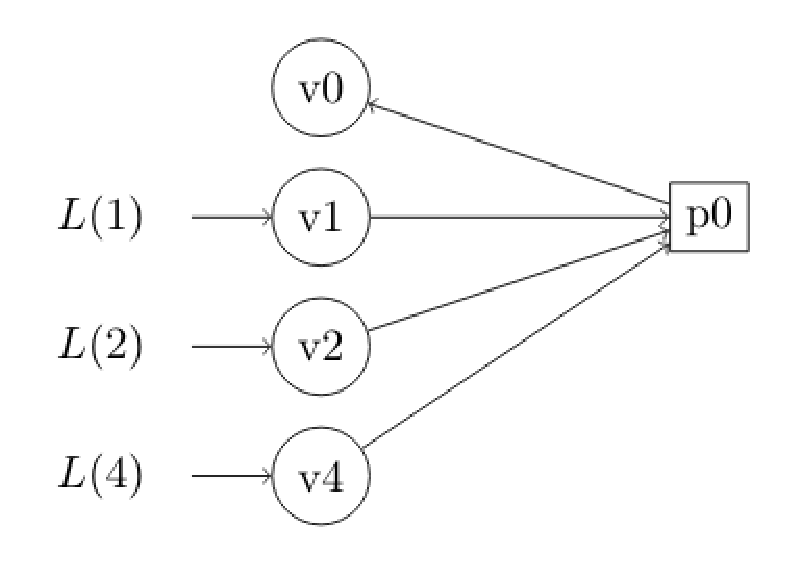
\includegraphics[width=\columnwidth]{./figs/checkope}
\end{center}
\caption{Check node operation}
\label{fig : check}
\end{figure}
since parity node equation for the first check node is $p_0=m_0+m_1+m_2+m_4$. we need to calculate
\begin{equation}\label{eq:sub}
\log \brak{\frac{1-\frac{1-p_0}{p_0}}{1-\frac{1-p_0}{p_0}}}
\end{equation}
Where $p_i$ is the probability. getting message from check to variable node by taking all variable node informations.
\begin{align}
\frac{1-\frac{1-p_0}{p_0}}{1-\frac{1-p_0}{p_0}} & = \frac{1-\frac{1-p_1}{p_1}}{1-\frac{1-p_1}{p_1}} \times \frac{1-\frac{1-p_2}{p_2}}{1-\frac{1-p_2}{p_2}} \times \frac{1-\frac{1-p_4}{p_4}}{1-\frac{1-p_4}{p_4}}\\
\frac{1-e^{-L_{ext0,0}}}{1+e^{-L_{ext0,0}}} &=\frac{1-e^{-L_{ext1,0}}}{1+e^{-L_{ext1,0}}}\times \frac{1-e^{-L_{ext2,0}}}{1+e^{-L_{ext2,0}}} \times \frac{1-e^{-L_{ext4,0}}}{1+e^{-L_{ext4,0}}}\\ \nonumber
\tanh \brak{\frac{L{ext0,0}}{2}}& =\tanh \brak{\frac{L{ext1,0}}{2}}\tanh \brak{\frac{L{ext2,0}}{2}}\\ \label{eq :first}
&\tanh \brak{\frac{L{ext4,0}}{2}} 
\end{align}

by substituting \eqref{eq :first} in \eqref{eq:sub} we get,
\begin{align}
\log \tanh \brak{\frac{L{ext0,0}}{2}} & = \log \tanh \brak{\frac{L{ext1,0}}{2}} +  \log \tanh \brak{\frac{L{ext2,0}}{2}}\\
& + \log \tanh \brak{\frac{L{ext4,0}}{2}}\\
\end{align}
\begin{equation}
sign(L_{ext0,0})= sign(L_{ext1,0})sign(L_{ext2,0})sign(L_{ext4,0})\\
\end{equation}
\begin{align}
\tanh \brak{\frac{\abs{L_{ext0,0}}}{2}} &=\tanh \brak{\frac{\abs{L_{ext1,0}}}{2}}\tanh \brak{\frac{\abs{L_{ext2,0}}}{2}}\\
&\tanh \brak{\frac{\abs{L_{ext4,0}}}{2}}
\end{align}
Using minsum algorithm \cite{minsum}
\begin{align}
L(r_{j=0,i=0}) &= sign(L(1))\times sign(L(2))\times sign(L(4))\\ \nonumber
&\times \min \brak{\abs{L(1)},\abs{L(2)},\abs{L(4)}} \\\nonumber
&=\sbrak{\prod_{k \in V_j \setminus i} sign(L(q_{kj}))} \min_{k \in V_j \setminus i} \abs{L(q_{kj})}\\ \label{eq : rji}
\end{align}
%
\item Variable Node Operation :\\
Let ${C_i}$ denotes all the check nodes connected to $i^{th}$ variable node. The message from $i^{th}$ variable node to  $j^{th}$ check node given by,
\begin{figure}[!ht]
\begin{center}
%\begin{tikzpicture}
%
%    
%    \node[shape=circle,draw=black] (v0) at (0,3) {v0};
%
%    
%
%
%    \node[shape=rectangle,draw=black] (p0) at (2,4) {p0};
%    \node[shape=rectangle,draw=black] (p1) at (2,3) {p1};
%    \node[shape=rectangle,draw=black] (p2) at (2,2) {p2};
%
%\path [->] (v0) edge node[left] {} (p0);
%\path [<-] (v0) edge node[left] {} (p1);
%\path [<-] (v0) edge node[left] {} (p2);
%
%
%\path [->] (-1,3) edge node[left] {} (v0);
%
%\node[] at (-1.4,3) {$L(0)$};
%
%\end{tikzpicture}
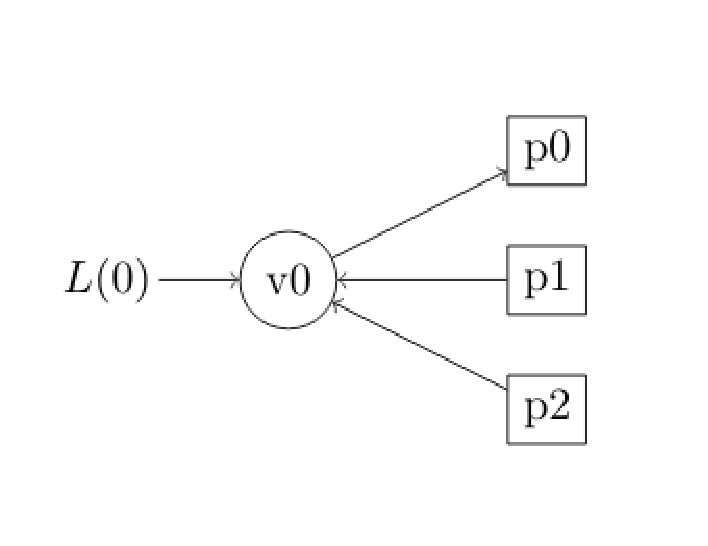
\includegraphics[width=\columnwidth]{./figs/varope}
\end{center}
\caption{Variable node operation}
\label{fig : var}
\end{figure}
\begin{align}
L(q_{i=0,j=0})&=\log \brak{\frac{Pr(x_j=1|y_0,y_1,y_2)}{Pr(x_j=-1|y_0,y_1,y_2)}} \quad X=1-2c\\
&= \log \brak{\frac{f(y_0,y1,y_2|x_j=1)Pr(x_j=1)}{f(y_0,y_1,y_2|x_j=-1)Pr(x_j=-1)}} \\
&= \log \brak{\frac{\frac{1}{\sqrt{2\pi\sigma^2}}e^{\frac{-(y_0-1)^2}{2\sigma^2}}\frac{1}{\sqrt{2\pi\sigma^2}}e^{\frac{-(y_1-1)^2}{2\sigma^2}}\frac{1}{\sqrt{2\pi\sigma^2}}e^{\frac{-(y_2-1)^2}{2\sigma^2}}}{\frac{1}{\sqrt{2\pi\sigma^2}}e ^{\frac{-(y_0+1)^2}{2\sigma^2}}\frac{1}{\sqrt{2\pi\sigma^2}}e ^{\frac{-(y_1+1)^2}{2\sigma^2}}\frac{1}{\sqrt{2\pi\sigma^2}}e ^{\frac{-(y_2+1)^2}{2\sigma^2}} }  } \\
&=\log \brak{e^{\frac{2(y_0+y_1+y_2)}{\sigma^2}}} \\
L(q_{i=0,j=0})&= \frac{2(y_0+y_1+y_2)}{\sigma^2}=L(x_i)+\sum_{k \in C_i\setminus j} L(r_{ki}) \label{eq: qij}
\end{align}
\end{enumerate}

\subsection{Message Passing Algorithm using min-sum Approximation}
Transmitted frames = N, Total number of bits = N $\times$ 7 and Total number of information bits = N $\times$ 4.
For Each Frame,
\begin{enumerate}
\item Initialize $L(q_{ij})$ using \eqref{eq :li} for all $i,j$ for which $h_{ij}=1$ with channel LLR's.
\item Update $\cbrak{L(r_{ji})}$ using \eqref{eq : rji}.
\item Update $\cbrak{L(q_{ji})}$ using \eqref{eq: qij}.
\item Update $\cbrak{L(V_i)}$ using,
\begin{equation}
L(V_i)=L(x_i)+\sum_{k \in C_i} L(r_{ki}) \quad i=0,\dots,6.
\end{equation}
\item Proceed to step 2.\\
After maximum specified iterations,

\end{enumerate}
Decoding can be done using,
\begin{equation}
\hat{c_i} = \begin{cases}
1 & L(V_i) < 0\\
0 & else
\end{cases}
\end{equation}
%
\section{Results}
For frames N=10000.
 \begin{figure}[!ht]
\begin{center}
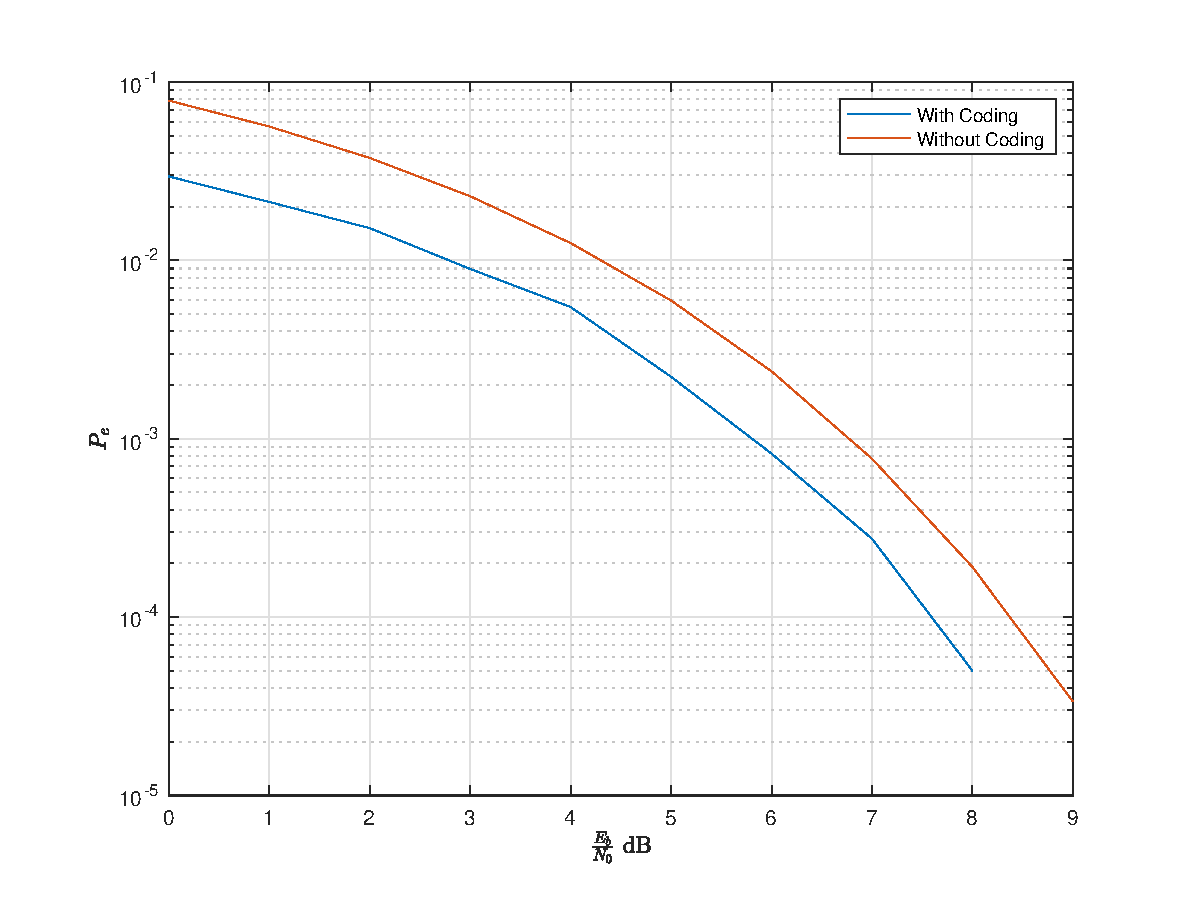
\includegraphics[width=\columnwidth]{./figs/ber}
\caption{SNR vs BER curves using LDPC channel coding and no channel coding}
\label{fig : ber}
\end{center}
\end{figure}
Fig \ref{fig : ber} Shows the Comparison of Probability error with channel coding and without channel coding. Since the parity check matrix taken was not much sparse, we are not getting near shannon limit performance. (Good sparse matrix i.e number of entries in H $<< m\times n $ )

\bibliography{IEEEabrv,ldpc.bib}
\end{document}

